%Part of/Parte di https://github.com/f-dinucci/appuntiMeccanicaFluidi/
%License/Licenza Creative Commons Attribution-ShareAlike 4.0 International (CC BY-SA 4.0) - attribution/attribuzione Francesco Di Nucci
%See also/Vedere anche https://creativecommons.org/licenses/by-sa/4.0/ and/e https://creativecommons.org/licenses/by-sa/4.0/legalcode
%
\section{Perdite di carico} 
%SUBSECTION
\subsection{Sforzo alla parete e perdita di carico}
Si può stimare la perdita di carico in un condotto con moto turbolento.
 %
	\begin{figure}[ht]
		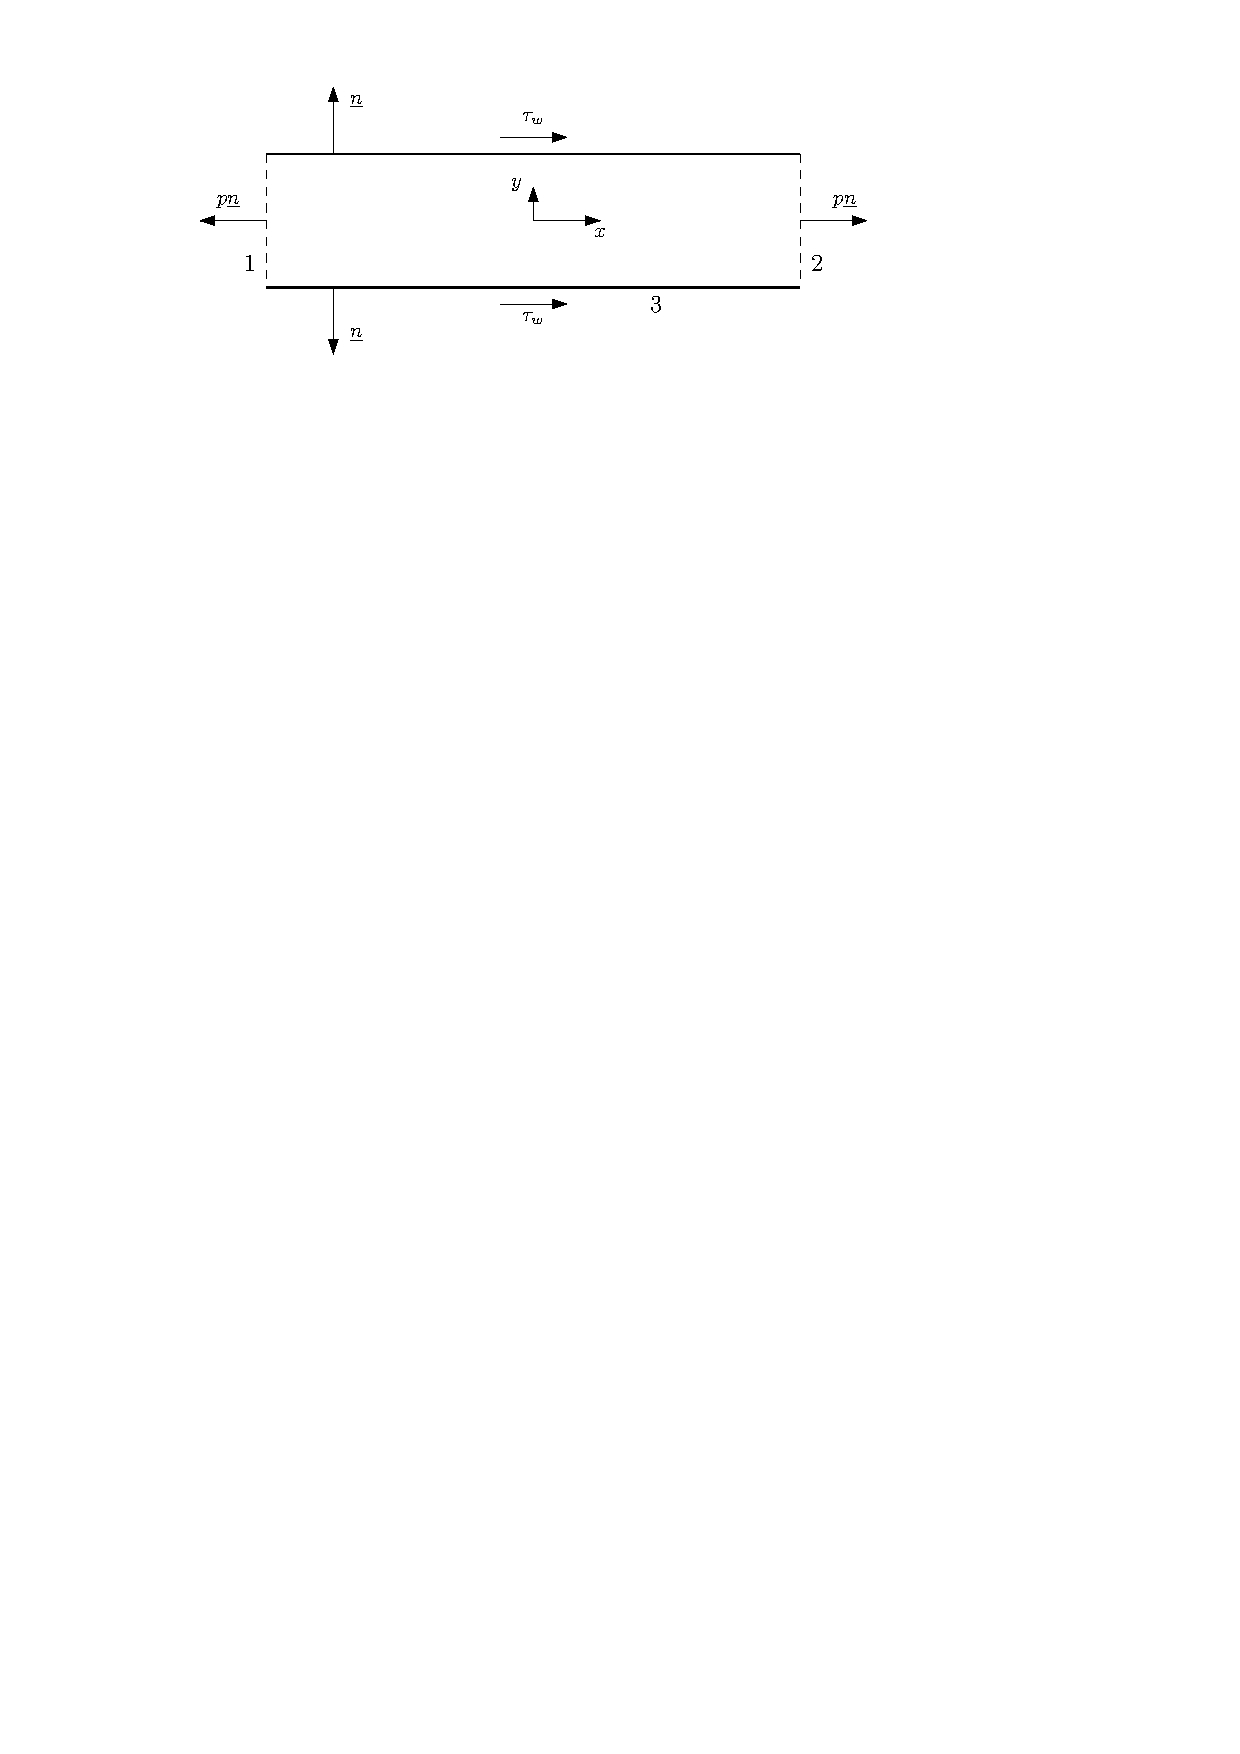
\includegraphics[scale=0.7]{./8.4 Perdite di carico/8.4-1}
		\centering
		\caption{Condotto e perdita di carico}
	\end{figure}
% 
Si parte dal bilancio di quantità di moto:
%
	\begin{equation*}
		\hat{\uline{x}} \vdot \int_1 \uuline{J}_Q \vdot \uline{n} \dd{S} + \hat{\uline{x}} \vdot \int_2 \uuline{J}_Q \vdot \uline{n} \dd{S} + \hat{\uline{x}} \vdot \int_3 \uuline{J}_Q \vdot \uline{n} \dd{S} = 0
	\end{equation*}
%
Dato che le velocità $u$ sono uguali ambo i lati se il flusso non dipende da $x$:
%
	\begin{equation*}
		- \int_1 (\cancel{\rho u^2} + p) \dd{S} + \int_2 (\cancel{\rho u^2}  + p)\dd{S} + \int_3 \tau_w \dd{S} = 0
	\end{equation*}
%
È una relazione sempre valida, dato che è ricavata dal bilancio di quantità di moto.
Detti $A$ l'area di base e $PL$ il prodotto perimetro per lunghezza:
%
	\begin{equation*}
		A (p_2 - p_1) + P L \tau_w = 0
	\end{equation*}
%
Da cui noto $\tau_w$ si trova la perdita di carico:
%
	\begin{equation*}
		p_1 - p_2 = L \frac{p}{A} \tau_w
	\end{equation*}
%

In particolare per un cerchio si ha che:
%
	\begin{equation*}
		\begin{gathered}
			\frac{A}{P} = \frac{\pi R^2}{2 \pi R} = \frac{R}{2} = \frac{D}{4}\\
			p_1 - p_2 = \frac{4 L}{D} \tau_w
		\end{gathered}
	\end{equation*}
%

%SUBSECTION
\subsection{Forma qualsiasi e caso piano}
\subsubsection{Forma qualsiasi}
Per una forma qualsiasi si calcola $D_H$, il diametro equivalente tale che valga la seguente relazione:
%
	\begin{equation*}
		\begin{gathered}
			D_H = \frac{4 A}{P}\\
			p_1 - p_2 = \frac{4L}{D_H} \tau_w
		\end{gathered}
	\end{equation*}
%

\subsubsection{Caso piano}
 %
	\begin{figure}[ht]
		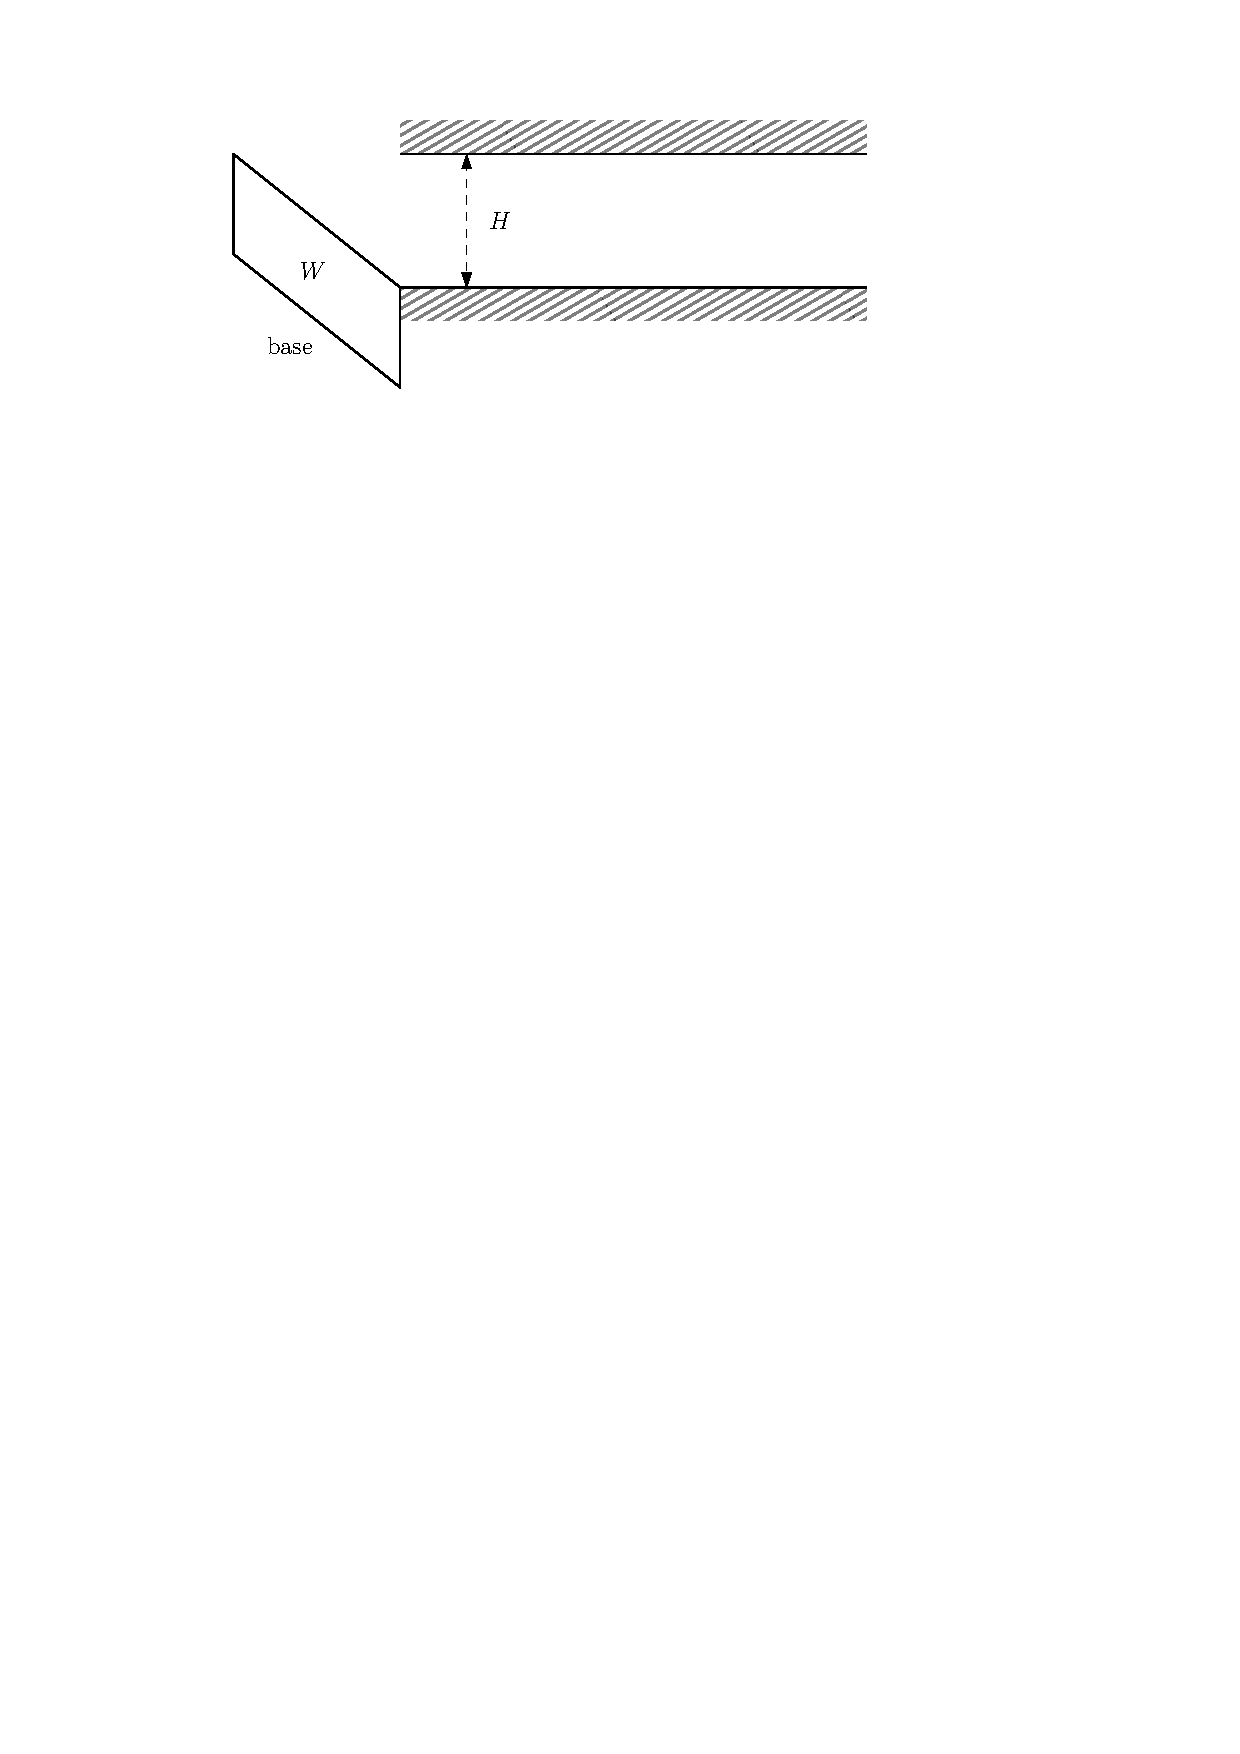
\includegraphics[scale=0.7]{./8.4 Perdite di carico/8.4-2}
		\centering
		\caption{Caso piano}
	\end{figure}
%
In questo caso si ha che:
%
	\begin{equation*}
		D_H = \frac{4 H W}{2 W} = 2H
	\end{equation*}
%
Poi si possono adimensionalizzare le formule di prima, definendo $f$ come fattore/coefficiente che lega perdita di carico e coefficiente di attrito:
%
	\begin{equation*}
		\begin{gathered}
			2 \frac{p_1 - p_2}{\rho \bar{u}^2} = \frac{L}{D_H} 4 \left( \frac{2 \tau_w}{\rho \bar{u}^2} \right)\\
			p_1 - p_2 = f \frac{L}{D_H} \rho \frac{\bar{u}^2}{2} \rightarrow f = 4 C_f
		\end{gathered}
	\end{equation*}
%


\subsection*{Bibliografia 8.4}
\cite[Cap.\ 12.4, 12.6]{PnueliGutfinger}